% The two interaction patterns of Lemma 3.4 for k = 5. Thick: the queried edge i = uu'.
% Dashed: the interacting coordinate j. Solid: edges that must be present.
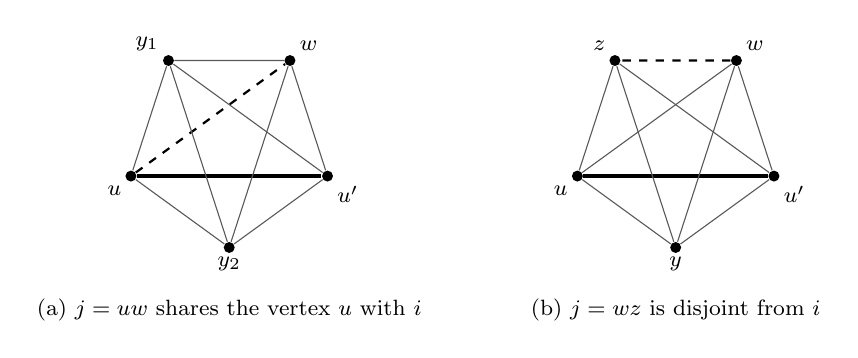
\begin{tikzpicture}[scale=1.05,
  v/.style={circle,fill=black,inner sep=1.4pt},
  lab/.style={font=\footnotesize},
  q/.style={very thick},
  j/.style={dashed,thick},
  e/.style={gray!70!black}]
  \begin{scope}
    \foreach \n/\a in {u/198,v/342,w/54,y1/126,y2/270} {\node[v] (\n) at (\a:1.25) {};}
    \node[lab,below left] at (u) {$u$}; \node[lab,below right] at (v) {$u'$};
    \node[lab,above right] at (w) {$w$}; \node[lab,above left] at (y1) {$y_1$};
    \node[lab,below] at (y2) {$y_2$};
    \draw[q] (u) -- (v);
    \draw[j] (u) -- (w);
    \foreach \a/\b in {u/y1,u/y2,v/w,v/y1,v/y2,w/y1,w/y2,y1/y2} {\draw[e] (\a) -- (\b);}
    \node[lab] at (0,-2.0) {(a) $j = uw$ shares the vertex $u$ with $i$};
  \end{scope}
  \begin{scope}[xshift=5.4cm]
    \foreach \n/\a in {u/198,v/342,w/54,z/126,y/270} {\node[v] (\n) at (\a:1.25) {};}
    \node[lab,below left] at (u) {$u$}; \node[lab,below right] at (v) {$u'$};
    \node[lab,above right] at (w) {$w$}; \node[lab,above left] at (z) {$z$};
    \node[lab,below] at (y) {$y$};
    \draw[q] (u) -- (v);
    \draw[j] (w) -- (z);
    \foreach \a/\b in {u/w,u/z,u/y,v/w,v/z,v/y,w/y,z/y} {\draw[e] (\a) -- (\b);}
    \node[lab] at (0,-2.0) {(b) $j = wz$ is disjoint from $i$};
  \end{scope}
\end{tikzpicture}
